\chapter{Aplicación de Prueba \label{chap:dummy_application}}
Con la finalidad de comprobar que \rc{} funciona de la manera esperada, se construyó una aplicación sencilla que use
esta librería. Además
de servir como prueba del software construido, también sirve como ejemplo de elaboración de aplicaciones sobre \rc.

Esta aplicación de prueba utiliza la mayoría de los artefactos de \rc, por lo que su ejecución permitió depurar los errores encontrados en
la etapa de \textit{testing}.

\section{Descripción del Problema}
\label{app_desc_problem}

Dada una lista de números enteros y un número a buscar, se desea saber si este último se encuentra en la lista. La complejidad de este
problema es muy baja, no obstante, lo que se deseaba era observar el comportamiento de la librería y la aplicación en cuanto a:
\begin{itemize}
    \item   distribución de tareas,
    \item   política de distribución sigmoidea,
    \item   fluidez entre servidor y clientes,
    \item   tiempo de corrida de la aplicación distribuida vs. secuencial, y
    \item   performance general del proyecto.
\end{itemize}


\section{Solución}

Esta aplicación, como ya dijimos, se trata de un simple algoritmo de búsqueda, con la particularidad de encontrar una solución que respete
la interfaz que \rc{} propone, y con esto aprovechar el poder de cómputo distribuido en varios nodos de procesamiento. Por ello, la solución
fue planteada siguiendo estos puntos:
\begin{enumerate}
    \item   Crear el \textit{functor} del problema, o sea especificar los atributos necesarios para poder resolver el problema de manera
            aislada. También debemos implementar el algoritmo que dado un functor nos dé $N$ functores hijos, cada uno de ellos más simple
            que el original.
    \item   Dar la implementación de serialización y deserialización del \textit{functor}.
    \item   Crear el \textit{functor} inicial, detallando así el estado del problema original.
    \item   Manejo de resultados.
\end{enumerate}

El algoritmo del punto 1 se realiza de esta manera porque debemos construir una solución que adopte la forma recursiva, ya que la librería
construida lo requiere. Con respecto a los 3 puntos restantes, se deben hacer estas operaciones por separado debido a que algunas serán
responsabilidades del servidor y otras del cliente. El cliente debe saber como un functor se divide en otros functores para llegar tarde o
temprano a los casos bases de cada functor, y por ende, enviar los resultados obtenidos. También debe conocer como se serializan y
deserializan los functores. En cambió, el servidor debe conocer cuál es el functor inicial, ya que es el encargado de iniciar la ejecución,
así como también saber reducir los resultados entrantes.


\subsection{Construcción del \textit{functor}}

Debe reflejar el estado del problema a resolver. En esta aplicación sólo necesitamos tener:
\begin{itemize}
    \item   la lista de números enteros, y
    \item   el número que se desee buscar.
\end{itemize}
Estos atributos son necesarios para solucionar el problema, ambos son requeridos como parámetros de entrada en el algoritmo de búsqueda. El
código fuente en \ref{middle_search} muestra la representación (como clase) creada para este functor, llamada
\texttt{MiddleSearch}.\\

\begin{table}[ht]
    \lstset{language=C++}
    \begin{lstlisting}[frame=single]
/** 
 * Class that represent the Middle Search recursive process.
 */
class MiddleSearch : public recabs::SerializableRecursiveFunctor
{

    public:
        
        typedef std::list<uint32_t> Elements;

        /** Standar constructor
         * 
         * @param v : Container of elements.
         * @param s : Item to search.
         */
        MiddleSearch(Elements& v, uint32_t s);

        /**
         * Destructor.
         */
        ~MiddleSearch(){};

        /**
         * Fills the list with its two children functors if the list
         * contains at least two elements. Otherwise, constructs the
         * corresponding package with the result.
         *
         * @param children : the list of RecursiveFunctor to fill,
         *                   in inductive case.
         * @param result : the packaging result to fill, in base case
         *                 or inductive case.
         *
         */
        virtual void call(ChildrenFunctors& children, Packet& result);

        /**
         * Serializes a MiddleSearch as a packet.
         *
         * @parram packet: Package that will be serialized itself.
         */        
        virtual void serialize(recabs::Packet& pkt);

    private:


        Elements _v;
        uint32_t _searched;

};
    \end{lstlisting}
    \centering
    \caption{Representación del functor}
    \label{middle_search}
\end{table}

La generación de functores hijos a partir de un functor (padre) es una operación de auto-reproduccción, ésto es, dado un functor, ser capaz
de generar functores más pequeños con la finalidad de llegar al caso base en una cantidad finita de ejecuciones por cada functor.

En este caso concreto, de un padre obtendremos dos hijos: un functor que contiene la mitad izquierda de la lista y otro con la derecha. Se
muestra un ejemplo en la figura \ref{functors_division_list} sobre la división de un functor en dos functores hijos.\\

\begin{figure}[ht]
    \begin{center}
        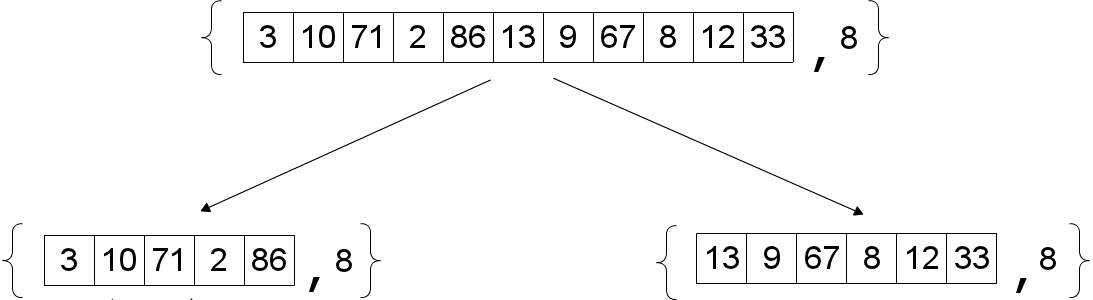
\includegraphics[scale=.35]{images/functors_division_list.png}
        \caption{Auto-reproducción de un functor}
        \label{functors_division_list}
    \end{center}
\end{figure}

El algoritmo utilizado para la división del functor fue el siguiente:
\begin{itemize}
    \item   Casos bases.
            \begin{itemize}
                \item   Si la lista es vacía, se envía un resultado con el valor de verdad \texttt{falso} al servidor.
                \item   Si la lista tiene un sólo elemento, se compara si este elemento es igual al número buscado y se envía el valor de
                        verdad correspondiente al servidor.
            \end{itemize}
    \item   Parte inductiva.
            \begin{enumerate}
                \item   Se descompone la lista de números en dos mitades.
                \item   Con ambas mitades se crean dos nuevos functores, los cuáles representan el mismo problema con diferentes entradas.
            \end{enumerate}
\end{itemize}

El código fuente perteneciente a este algoritmo se encuentra en \ref{call_middle_search}. Para visualizar como continúa la división
de functores del ejemplo graficado en \ref{functors_division_list}, véase la figura \ref{middle_search_tree} que muestra el gráfico
completo sobre la misma lista.

\begin{table}[ht]
    \lstset{language=C++}
    \begin{lstlisting}[frame=single]
void Functor::call(ChildrenFunctors& children, Packet& result)
{
    /* Base case 1 */
    if (_v.empty())
    {
        mili::bostream bos;
        bos << false;
        result = bos.str();
    }

    /* Base case 2 */
    if (uint32_t (_v.size()) == 1)
    {
        mili::bostream bos;
        bos << (_v.front() == _searched);
        result = bos.str();
    }
    /* Inductive case */
    else
    {
        Elements::iterator it = _v.begin();
        advance(it, _v.size() / 2);

        Elements leftChild(_v.begin(), it);
        Elements rightChild(it++, _v.end());

        insert_into(children, new BinarySearch(leftChild, _searched));
        insert_into(children, new BinarySearch(rightChild, _searched));
    }
}
    \end{lstlisting}
    \centering
    \caption{Código para la reproducción de functores}
    \label{call_middle_search}
\end{table}

\subsection{Serialización y Deserialización}

Un functor debe poder serializarse para ser enviado por la red y al llegar a un cliente, éste debe deserializarlo para luego procesarlo.
Para llevar a cabo estas dos operaciones se hizo uso de la librería MiLi\footnote{http://code.google.com/p/mili/}, más específicamente el
módulo \texttt{mili::binary\_streams} el cuál se encarga de crear \textit{streams} binarios con los atributos que tenga el functor.

En \ref{serialize_middle_search} se muestra el código para la serialización  y en \ref{deserialize_middle_search} para la deserialización de
un functor. La serialización consistió en insertar primero la lista de números y luego el número a buscar en la lista. Obviamente cuando
deserializamos hacemos las operaciones inversas al serializado.

\begin{table}[ht]
    \lstset{language=C++}
    \begin{lstlisting}[frame=single]
void Functor::serialize(Packet& pkt)
{
    mili::bostream bos;
    bos << this->_v << this->_searched;
    pkt = bos.str();
}
    \end{lstlisting}
    \centering
    \caption{Serialización del functor}
    \label{serialize_middle_search}
\end{table}

\begin{table}[ht]
    \lstset{language=C++}
    \begin{lstlisting}[frame=single]
void MSDeserializer::deserialize(const Packet& pkt, Functor** rf)
{
    mili::bistream bis(pkt);

    uint32_t searched;
    MiddleSearch::Elements v;
    bis >> v >> searched;
    *rf = new MiddleSearch(v, searched);
}
    \end{lstlisting}
    \centering
    \caption{Deserialización del functor}
    \label{deserialize_middle_search}
\end{table}

\subsection{\textit{Functor} inicial}

Para que el server pueda iniciar la ejecución de la solución, es necesario que disponga del functor inicial, el cuál contiene los datos
originales de entrada, o sea la lista total de números enteros. Para la creación del paquete inicial, primero se debe usar el método
de construcción y luego el de serialización, como se muestra en el código exhibido en \ref{init_middle_search}.

Este aplicación se configuró con un functor inicial que contiene una lista de un millón de números enteros, la cuál es $[0, 1, 2, ...,
999999]$ y el número a buscar es el $-1$.

\begin{table}[ht]
    \lstset{language=C++}
    \begin{lstlisting}[frame=single]
void L4ServerMS::get_initial_packet(Packet& pkt)
{
    MiddleSearch::Elements v;

    for (uint32_t i = 0; i < 1000000; i++)
        mili::insert_into(v, i);

    MiddleSearch b(v, -1);

    b.serialize(pkt);
}
    \end{lstlisting}
    \centering
    \caption{Creación del functor inicial}
    \label{init_middle_search}
\end{table}

\subsection{Manejo de resultados}

El servidor debe tener un algoritmo que maneje los resultados que llegan desde los clientes, los cuáles procesan sus functores y, por
ende, generan y envían estos resultados en base a sus propios cómputos.

En \ref{result_middle_search} se muestra el código fuente que reduce los resultados con la operación lógica \textbf{OR}, debido a que si
\textit{al menos un} functor encuentra el número buscado en la lista, devolveremos {verdadero}. Por contraparte, el número no estará en la
lista si \textit{todos} los functores devuelven el valor de verdad \texttt{falso}.

\begin{table}[ht]
    \lstset{language=C++}
    \begin{lstlisting}[frame=single]
void L4ServerMS::receive_result(const Packet& pkt)
{
    mili::bistream bis(pkt);
    bool res;
    bis >> res;

    _result = (_result || res);
}
    \end{lstlisting}
    \centering
    \caption{Manejo de resultados}
    \label{result_middle_search}
\end{table}


\section{Árbol de functores}
\label{functors_tree}

En toda aplicación podemos ver como los functores forman un árbol que comienza con el functor inicial, luego se van creando los hijos, y
así sucesivamente. Cabe aclarar que cada functor de este árbol va a ser procesado por un cliente en particular, apoyándose en otros
clientes para poder distribuir todos los functores, y así aprovechar al máximo los clientes disponibles del sistema.

En la figura \ref{middle_search_tree} se muestra un ejemplo de árbol de functores para esta aplicación en particular, la cuál tiene como
número a buscar el $8$, y el functor inicial con la siguiente lista: $[3, 10, 71, 2, 86, 13, 9, 67, 8, 12, 33]$.

\begin{center}
    \begin{landscape}
        \begin{figure}[ht]
            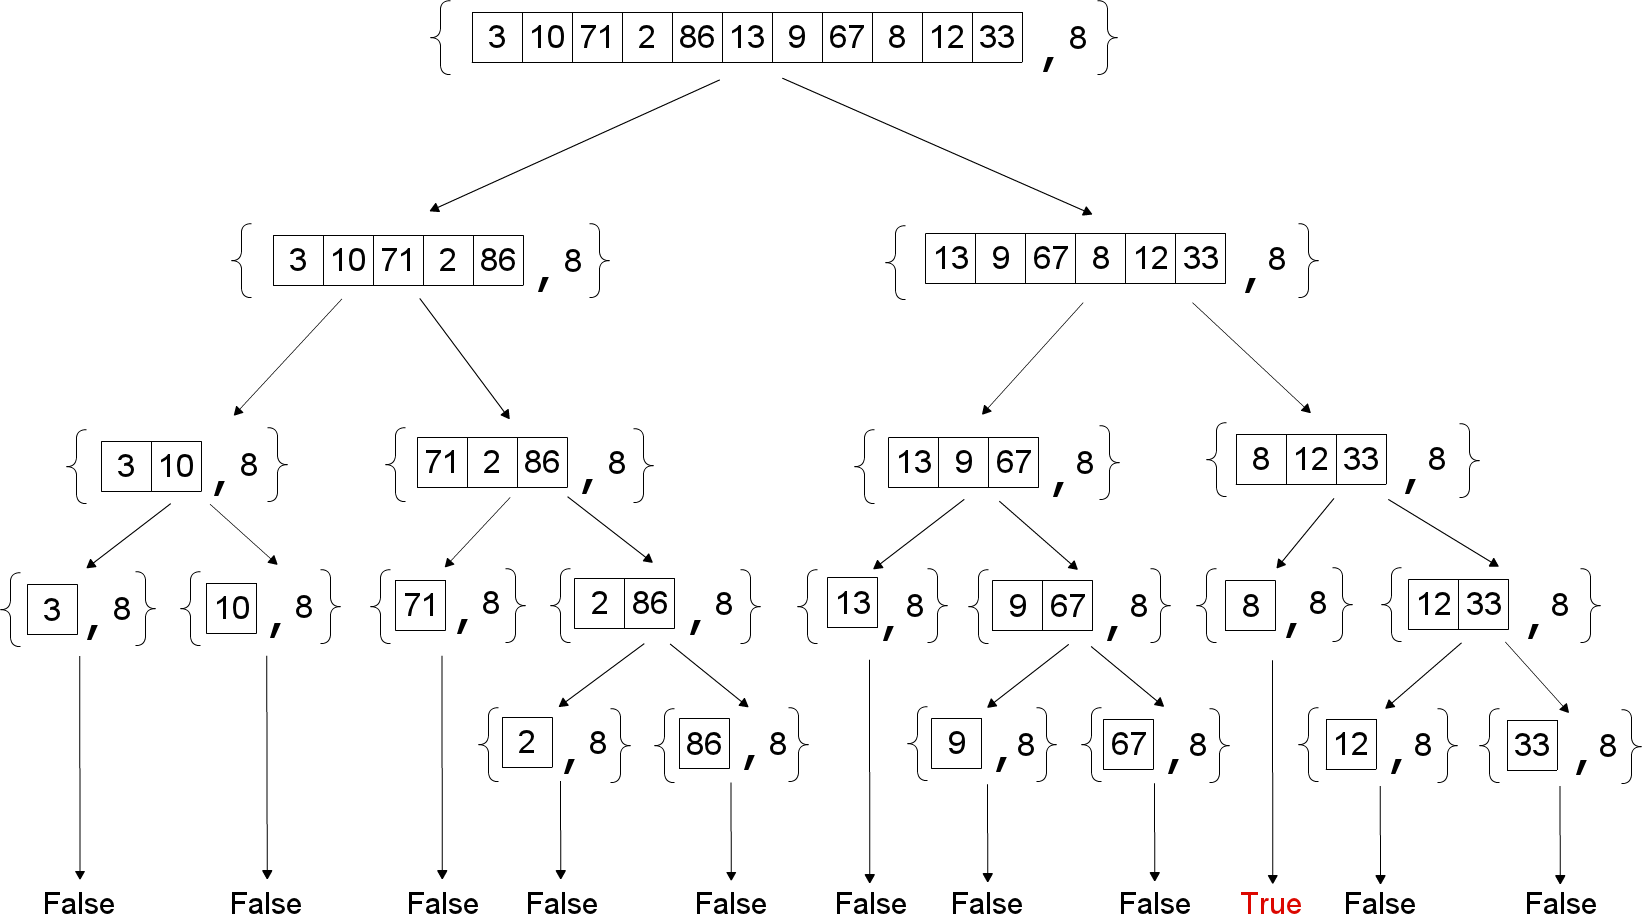
\includegraphics[scale=.37]{images/middle_search_tree.png}
            \caption{Ejemplo de árbol de functores generado por la aplicación de prueba}
            \label{middle_search_tree}
        \end{figure}
    \end{landscape}
\end{center}


\section{Análisis de performance}

Un algoritmo secuencial es usualmente evaluado en términos de su tiempo de ejecución, expresado como una función de su tamaño de entrada. El
tiempo de ejecución de la versión distribuida depende no sólo del tamaño de la entrada sino también del número de nodos usados, y el costo
de comunicación entre nodos.\\

Es importante estudiar la performance de un programa distribuido con el propósito de compararlo con su versión secuencial y así analizar
sus beneficios. Para ello se cuenta con métricas, las cuales nos arrojarán resultados o indicadores sobre el análisis de la performance de
un programa.\\

A continuación mostraremos las principales métricas de este algoritmo de búsqueda distribuido y sus correspondientes análisis, luego de
haber ejecutado el programa con una lista de $10000000$ de elementos con distintas cantidades de nodos de procesamiento. La definición de
estas métricas de rendimiento se encuentran en el libro de \textit{Ian Foster}\cite{parallel}.\\


\subsection{Tiempo de ejecución}

Tiempo de ejecución de un programa: es el intervalo de tiempo desde que el programa se inicia hasta que finaliza. En el caso de
computación distribuida un programa finaliza cuando el último nodo termina su ejecución.

Se denotará el tiempo de ejecución de la búsqueda implementada secuencialmente como $T_s$ y el tiempo de la versión distribuida como
$T_p$. El promedio de $T_s$ en diez ejecuciones fue de $185,77$ segundos.

%BoxPlot
Tomando como muestra diez ejecuciones por misma cantidad de clientes, se confeccionó en el gráfico \ref{execution_boxplot} los
\textit{boxplot's} para uno, dos, tres, cuatro y cinco nodos de procesamiento, respectivamente.
\begin{figure}[!ht]
    \begin{center}
        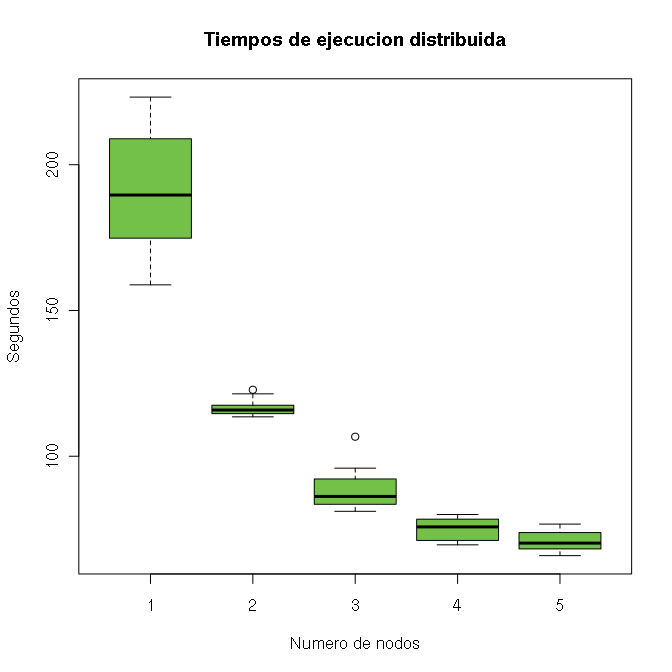
\includegraphics[scale=0.44]{images/execution_boxplot.png}
        \caption{Boxplot's de tiempo de ejecución distribuida}
        \label{execution_boxplot}
    \end{center}
\end{figure}

En la figura \ref{ts_vs_tp} se muestran los tiempos de ejecución promedio para uno a cinco clientes, así como su comparación con el
algoritmo secuencial.
 
\begin{figure}[!ht]
    %Tabla & Grafico
    \begin{minipage}{3cm}
    \begin{flushleft}
    \begin{tabular*}{2,5cm}{c@{\extracolsep{\fill}}c}
        \hline
        \textbf{p} & \textbf{$T_p$} \\ \hline 
        1 & 190,5 \\ \hline
        2 & 116,7 \\ \hline
        3 & 88,6 \\ \hline
        4 & 74,8 \\ \hline
        5 & 70,8 \\ \hline
    \end{tabular*}
    \end{flushleft}
    \end{minipage}
    \    \ \hfill
    \begin{minipage}{12cm}
    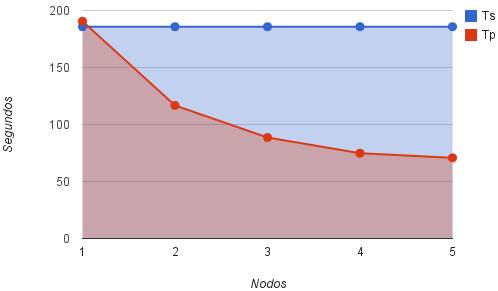
\includegraphics[scale=0.6]{images/ts_vs_tp.png}\\
    \end{minipage}
    \caption{Tiempo secuencial vs. paralelo}
    \label{ts_vs_tp}
\end{figure}

Visto estos resultados, se nota una mejora en rendimiento de tiempo entre la ejecución del programa secuencial y la versión distribuida
ejecutada sobre \rc. Cuando se ejecuta con menos de $3$ nodos (o clientes) podemos decir que el tiempo baja a gran escala pero cuando son
más de $3$, el tiempo de ejecución queda en una meseta.


\subsection{Overhead}

El \textit{overhead} de un programa paralelo es el trabajo adicional que dicho programa realiza respecto a la solución secuencial
equivalente, y se define como: $T_0 = p*T_p - T_s$ .

\begin{figure}[ht]
    %Tabla & Grafico
    \begin{minipage}{3cm}
    \begin{flushleft}
    \begin{tabular*}{2,5cm}{c@{\extracolsep{\fill}}c}
        \hline
        \textbf{p} & \textbf{$T_0$} \\ \hline 
        1  & 4,77 \\ \hline
        2  & 47,65 \\ \hline
        3  & 80,03 \\ \hline
        4  & 113,51 \\ \hline
        5  & 167,98 \\ \hline
    \end{tabular*}
    \end{flushleft}
    \end{minipage}
    \    \ \hfill
    \begin{minipage}{12cm}
    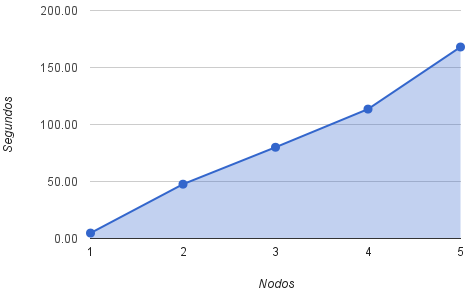
\includegraphics[scale=0.6]{images/overhead.png}\\
    \end{minipage}
    \caption{Overhead}
    \label{overhead}
\end{figure}

En la figura \ref{overhead} vemos que el overhead es directamente proporcional al número de procesadores, lo que indica mismo tiempo de
trabajo adicional por cliente agregado a la ejecución, respecto del algoritmo secuencial.
    

\subsection{Aceleración}

Cuando evaluamos un sistema distribuido, a menudo nos interesa conocer cuánto ganamos en performance paralelizando un algoritmo con respecto
a su implementación secuencial. La aceleración es una medida que arroja el beneficio relativo de resolver un problema en paralelo. Ésta
es definida como la relación del tiempo que toma resolver un problema en un sólo procesador con el tiempo requerido para resolverlo en una
arquitectura paralela con $n$ nodos de procesamiento idénticos. La aceleración se denota con el símbolo $S$ y se define como: $S=T_s/T_p$ .

\begin{figure}[ht]
    %Tabla & Grafico
    \begin{minipage}{3cm}
    \begin{flushleft}
    \begin{tabular*}{2,5cm}{c@{\extracolsep{\fill}}c}
        \hline
        \textbf{p} & \textbf{$S$} \\ \hline 
        1  & 0,97 \\ \hline
        2  & 1,59 \\ \hline
        3  & 2,10 \\ \hline
        4  & 2,48 \\ \hline
        5  & 2,63 \\ \hline
    \end{tabular*}
    \end{flushleft}
    \end{minipage}
    \    \ \hfill
    \begin{minipage}{12cm}
    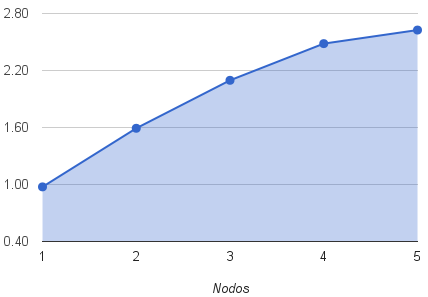
\includegraphics[scale=0.6]{images/speedup.png}\\
    \end{minipage}
    \caption{Aceleración}
    \label{speedup}
\end{figure}

Notemos que en el gráfico \ref{speedup}, la performance de la ejecución paralela aumenta en mayor medida hasta los 3 nodos, y luego el
rendimiento se estabiliza por más nodos que se agregue a la ejecución.


\subsection{Eficiencia}

La eficiencia es una medida que indica la fracción de tiempo útil de un elemento de procesamiento. Se denota con el símbolo $E$ y se
define como: $E = S/p$ .
      
\begin{figure}[ht]
    %Tabla & Grafico
    \begin{minipage}{3cm}
    \begin{flushleft}
    \begin{tabular*}{2,5cm}{c@{\extracolsep{\fill}}c}
        \hline
        \textbf{p} & \textbf{$E$} \\ \hline 
        1  & 0,97 \\ \hline
        2  & 0,80 \\ \hline
        3  & 0,70 \\ \hline
        4  & 0,62 \\ \hline
        5  & 0,53 \\ \hline
    \end{tabular*}
    \end{flushleft}
    \end{minipage}
    \    \ \hfill
    \begin{minipage}{12cm}
    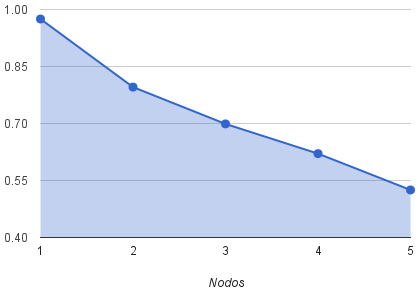
\includegraphics[scale=0.6]{images/eficiency.png}\\
    \end{minipage}
    \caption{Eficiencia}
    \label{eficiency}
\end{figure}

En la figura \ref{eficiency}, vemos que la función de eficiencia decae linealmente, lo que significa una utilidad nodal inversamente
proporcional a la cantidad de nodos procesantes.


\subsection{Costo}
      
El costo de un programa paralelo refleja la suma de los tiempos de ejecución de cada unidad de procesamiento. Se dice que un programa
paralelo tiene costo óptimo si tiene costo computacional igual al programa secuencial. Se define como: $C = p*T_p$ . Esta métrica esta
íntimamente relacionada con la comunicaciones entre los nodos.

\begin{figure}[ht]
    %Tabla & Grafico
    \begin{minipage}{3cm}
    \begin{flushleft}
    \begin{tabular*}{2,5cm}{c@{\extracolsep{\fill}}c}
        \hline
        \textbf{p} & \textbf{$C$} \\ \hline 
        1  & 190,54 \\ \hline
        2  & 233,42 \\ \hline
        3  & 265,80 \\ \hline
        4  & 299,28 \\ \hline
        5  & 353,75 \\ \hline
    \end{tabular*}
    \end{flushleft}
    \end{minipage}
    \    \ \hfill
    \begin{minipage}{12cm}
    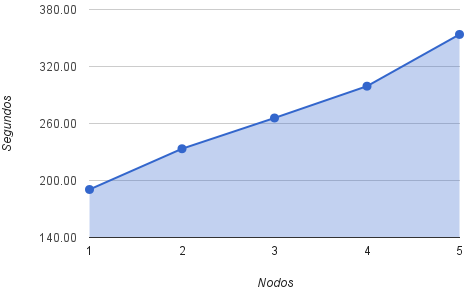
\includegraphics[scale=0.6]{images/cost.png}\\
    \end{minipage}
    \caption{Costo}
    \label{cost}
\end{figure}

En \ref{cost} véase que el costo tiene la misma curva que el overhead salvo el offset del tiempo del algoritmo secuencial. En este ejemplo,
se nota un costo proporcional a la cantidad de nodos.
